\documentclass[11pt, oneside]{article}   	% use "amsart" instead of "article" for AMSLaTeX format


\usepackage[letterpaper, top=10mm, left=22mm, right=22mm]{geometry}
             		% See geometry.pdf to learn the layout options. There are lots.
              		% ... or a4paper or a5paper or ... 
%\geometry{landscape}                		% Activate for rotated page geometry
%\usepackage[parfill]{parskip}    		% Activate to begin paragraphs with an empty line rather than an indent
\usepackage{graphicx}				% Use pdf, png, jpg, or eps§ with pdflatex; use eps in DVI mode
								% TeX will automatically convert eps --> pdf in pdflatex
\usepackage{amssymb,amsmath,multirow,subfigure}
  
\title{\bf HPC-Homework 2}
\author{\bf \large Ya Zhu}
\date{}							% Activate to display a given date or no date
\begin{document}
\maketitle 
\section{Bug fixing}
\begin{itemize}
\item omp\_bug2: \emph{tid} and \emph{total} should be declared private for each thread.
\item omp\_bug3: \emph{\#pragma omp barrier} should not be outside the parallel directives. So comment it.
\item omp\_bug4: $a[N][N]$ may be too large to store in thread stack space and cause segment fault. So change to a smaller N.
\item omp\_bug5: if one thread has set \emph{locka} while the other has set \emph{lockb}, then when they are trying to set the other lock, deadlock happened. So unlock the lock before setting another one.
\item omp\_bug6: reduction variable should be shared by all the threads executing \emph{dotprod}. So set \emph{sum} global, and then no return variable needed for \emph{dotprod}.
\end{itemize}
\section{Experiment}
\subsection{Settings}
\begin{itemize}
\item Machine: Courant server \emph{crunchy1} (64 cores).
\item Compiling option: -O3 for all methods.
\item The residual is the L2-norm (Euclidean norm): $||A\boldsymbol{u}^k-\boldsymbol{f}||=\sqrt{\sum_{i,j}({-\Delta_{u_{ij}}-f})^2}$.
\end{itemize}
\subsection{Results}
\subsubsection{Convergence}
For this problem, we have used three different methods: Jacobi2D, GS-red/black and GS-serial, where GS-red/black is the Gauss-Seidel method with red-black coloring while GS-serial does not use red-black coloring and parallelization. Figures 1 and 2 show the convergence behavior of the three methods with $N=\{24,100,500\}$. Figure 1 shows the relation between the residuals and the number of iterations, while Figure 2 shows relative residual-reductions (compare to the initial residual) along with the number of iterations. 

From Figure 1, we can see that the residuals of the GS-red/black method increase at the early iterations, and as $N$ becomes larger, GS-red/black takes more iterations to achieve the reduction of residual. However, after the early iterations, the GS-red/black converges faster than Jacobi2D as it was in 1D situation. While the GS-serial does not lead to residual-increase and hence converges faster than GS-red/black. From Figure 2, we can see that the convergence rate of two GS methods are similar and are twice as fast as Jacobi, which is consistent as the result of 1D Jacobi and Gauss-Seidel. These results imply that though Gauss-Seidel method using red-black coloring needs more iterations at the early stage to converge than the standard version, it still has good convergence behavior. Therefore, it is reasonable and beneficial to use GS-red/black to do parallelization.
\begin{figure}[ht]
\subfigure[$N=24$ \label{f1}]{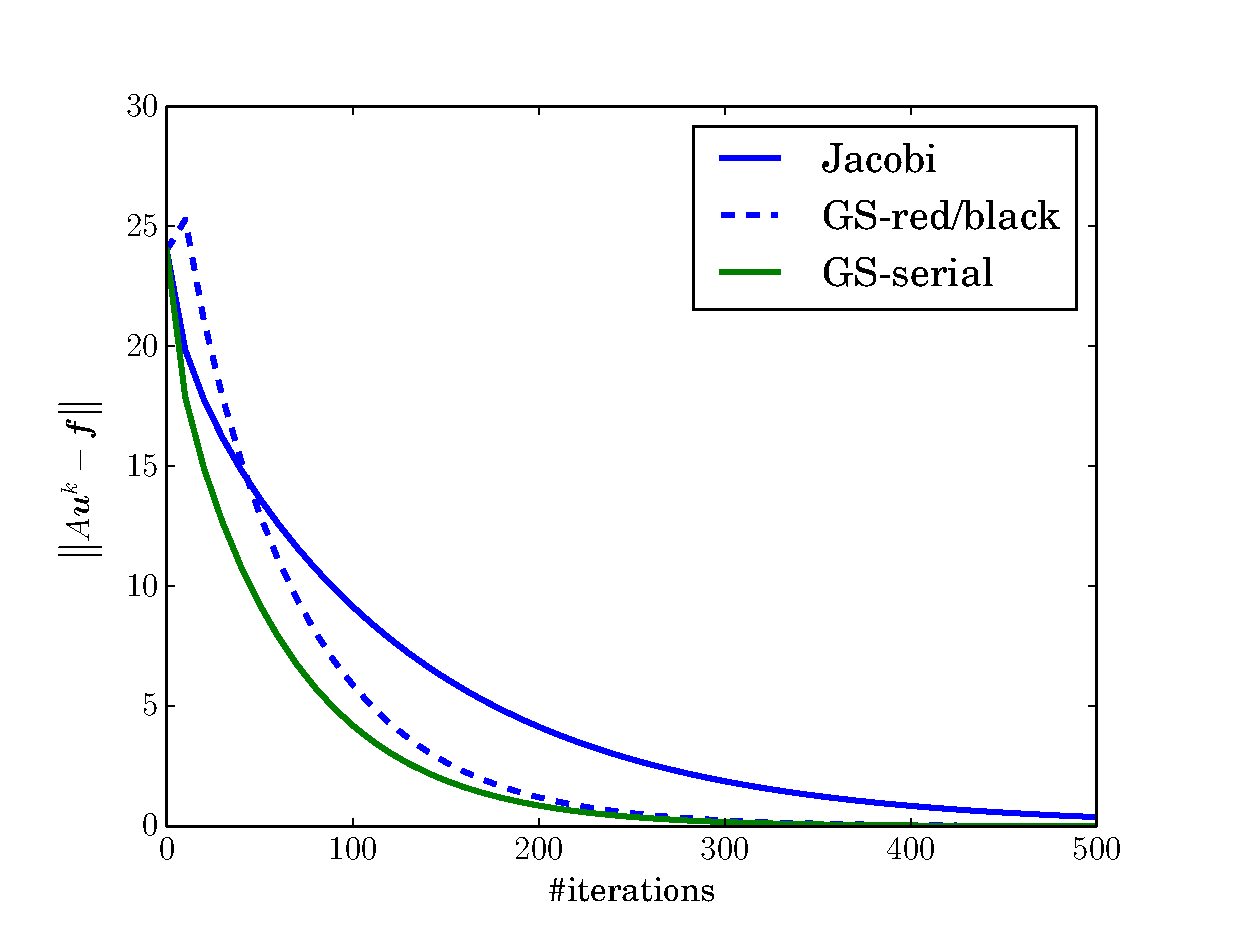
\includegraphics[width=0.33\linewidth]{figs/ri24.eps}}
\subfigure[$N=100$ \label{f2}]{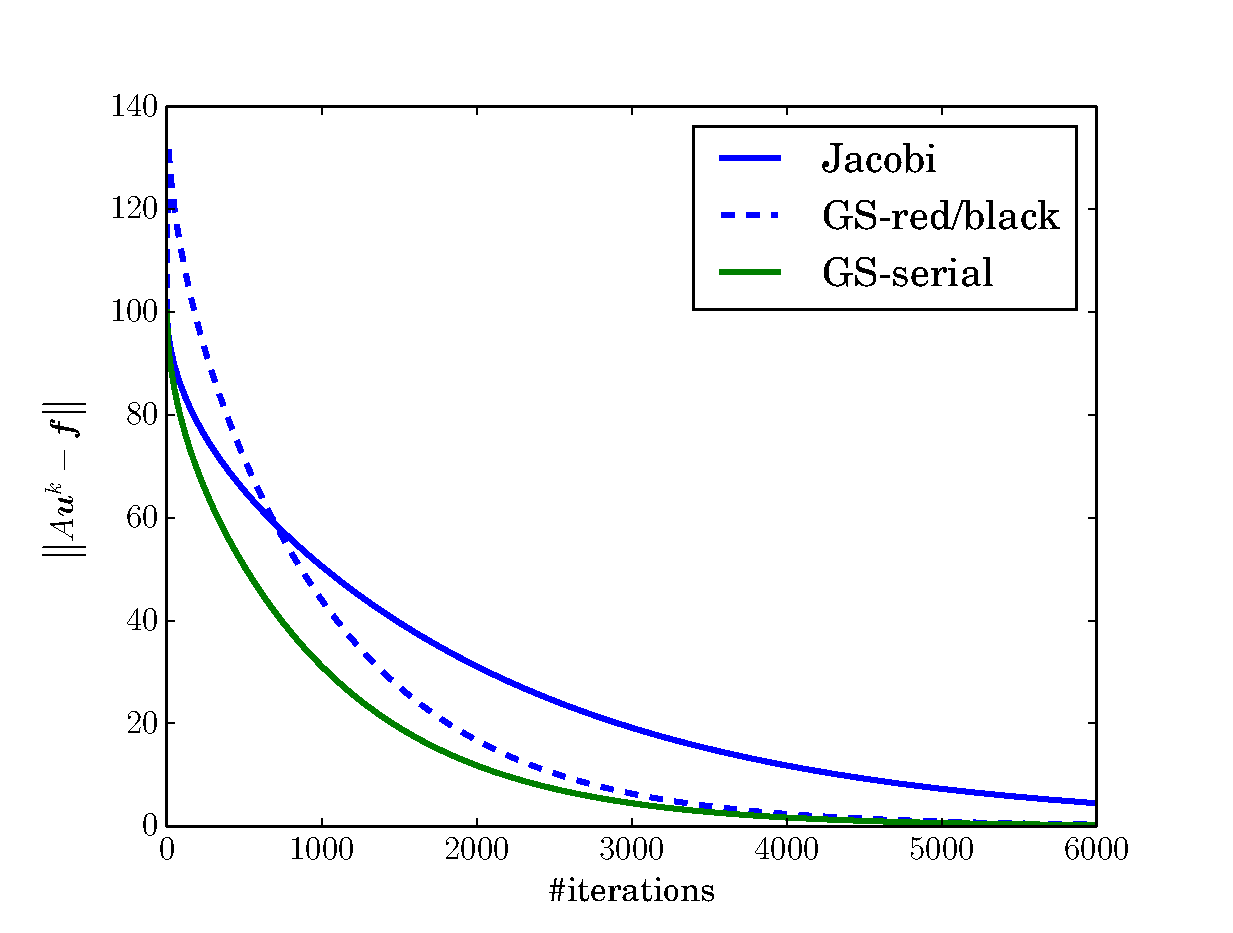
\includegraphics[width=0.33\linewidth]{figs/ri100.eps}}
\subfigure[$N=500$ \label{f2}]{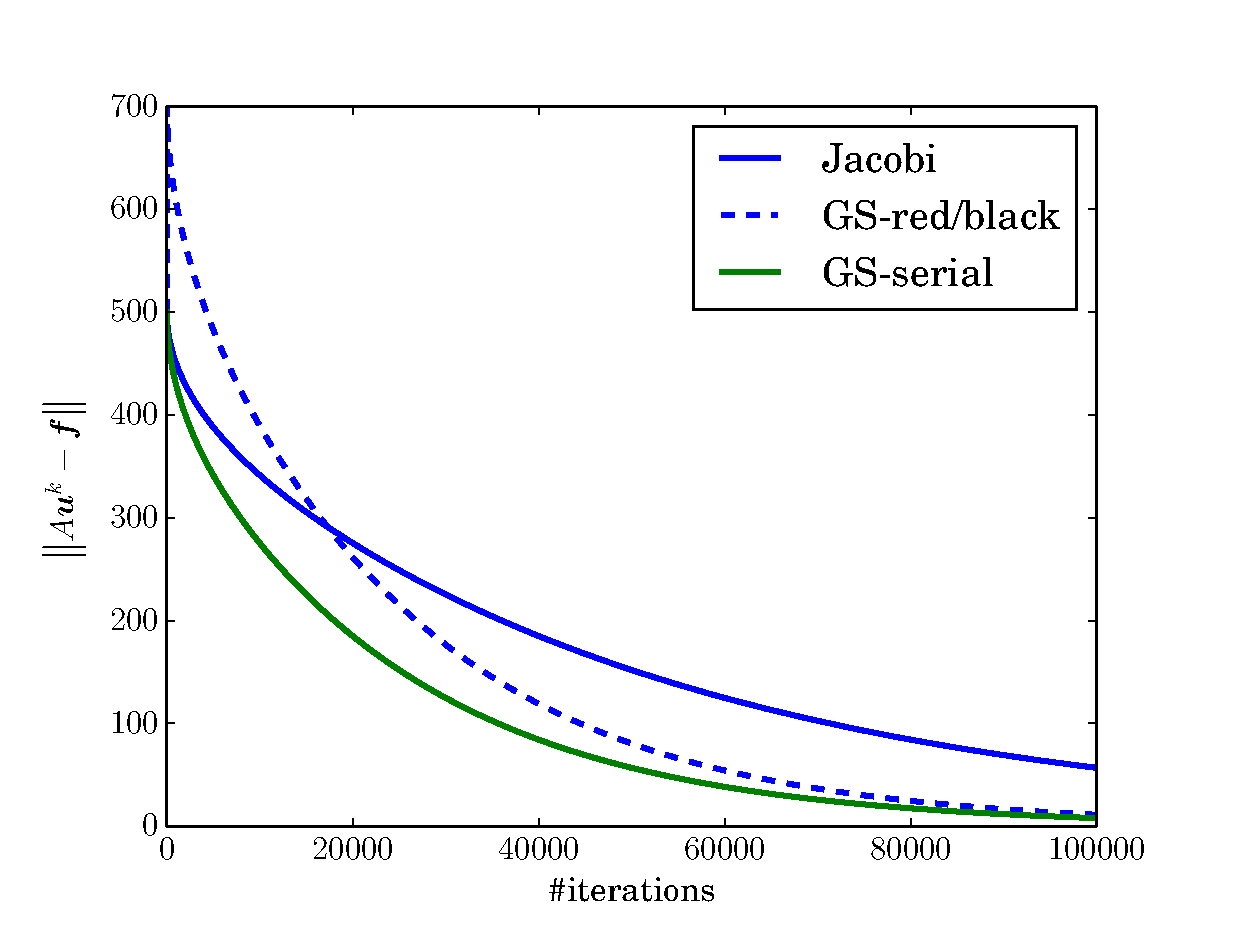
\includegraphics[width=0.33\linewidth]{figs/ri500.eps}}
\caption{Residuals vs. the number of iterations.}
\end{figure}
\begin{figure}[ht]
\subfigure[$N=24$ \label{f1}]{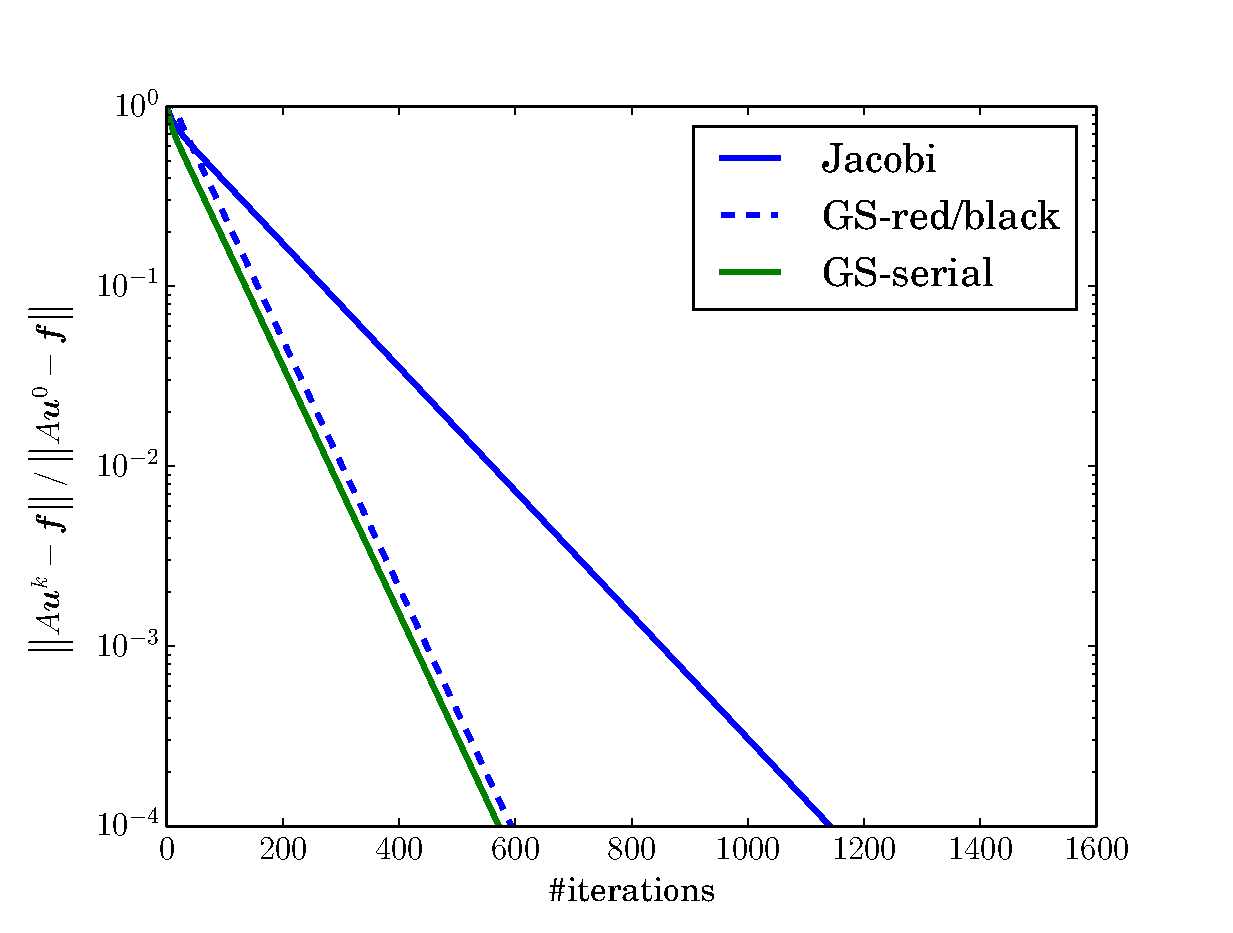
\includegraphics[width=0.33\linewidth]{figs/cg_24.eps}}
\subfigure[$N=100$ \label{f2}]{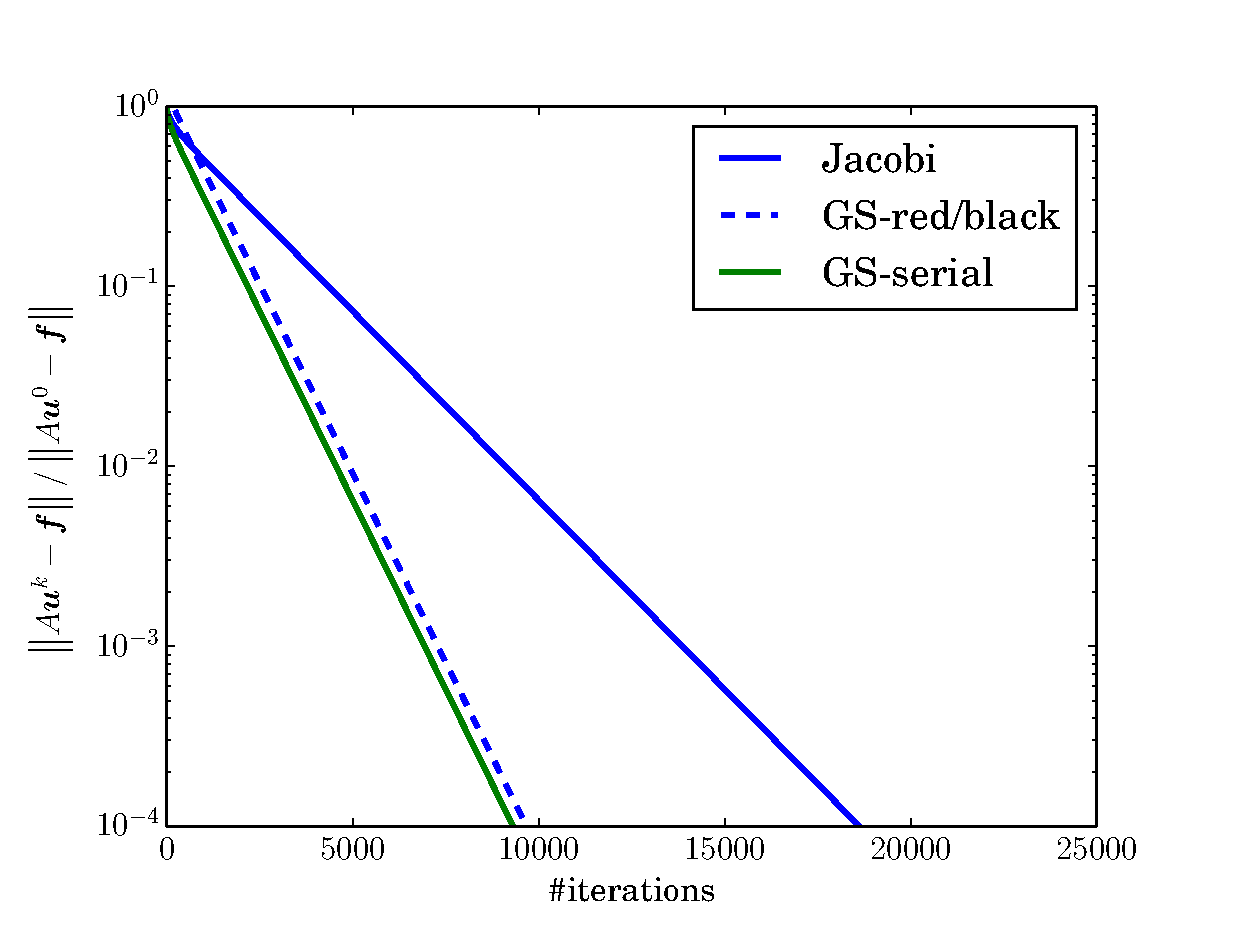
\includegraphics[width=0.33\linewidth]{figs/cg_100.eps}}
\subfigure[$N=500$ \label{f2}]{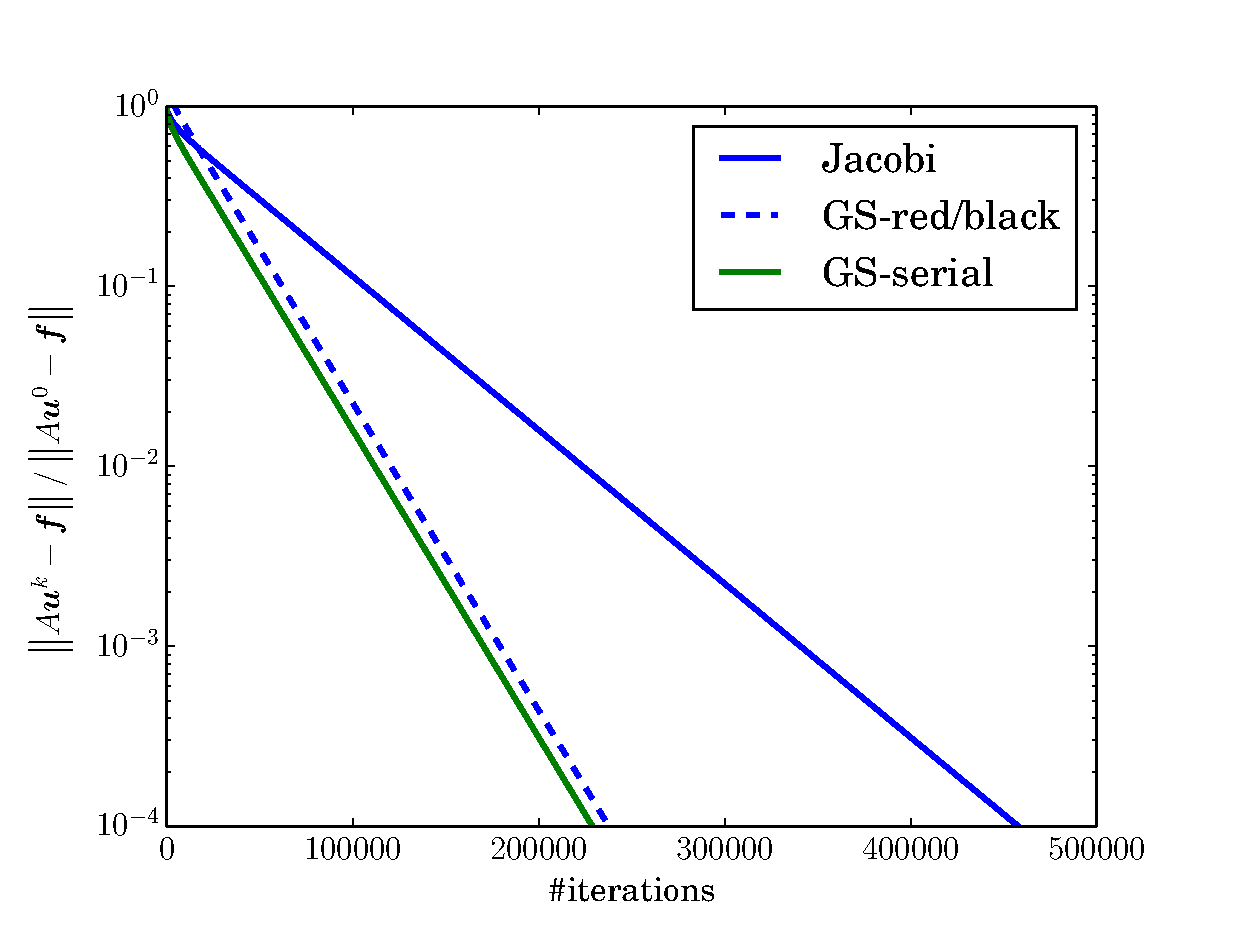
\includegraphics[width=0.33\linewidth]{figs/cg_500.eps}}
\caption{Relative residual-reductions vs. the number of iterations.}
\end{figure}
\subsubsection{Timing}
Table 1 shows the timing of two parallel methods for $N=500$ and $Iter= 100000$ with different number of threads. Note that experiment about timing is hard to conduct especially on public server with multiple processes running in it. However, we can still roughly conclude from the results that different numbers of threads lead to quite different running time the program need: could be nearly 10 times difference. For this case, though the machine has 64 cores in total, using too many threads (e.g., more than 24) results in very slow execution, while using 8 or 10 threads seems the best choice.
\begin{table}[ht]
\centering
\caption{Run time comparison of two methods with $N=500$ and $Iter= 100000$. (Unit: second)}
\begin{tabular}{|c|r|r|r|r|r|r|r|r|r|}
\hline
\#threads             & \multicolumn{1}{c|}{2} & \multicolumn{1}{c|}{4} & \multicolumn{1}{c|}{8} & \multicolumn{1}{c|}{10} & \multicolumn{1}{c|}{16} & \multicolumn{1}{c|}{24} & \multicolumn{1}{c|}{32} & \multicolumn{1}{c|}{48} & \multicolumn{1}{c|}{64} \\ \hline
jacobi2D-omp  & 279.76  & 134.76  & {\bf 79.01}  & 109.08   & 217.47   & 543.70   & 845.17   &  1101.78  & 1268.22   \\ \hline
gs2D-omp      &  141.77 & 73.51  & 57.86  &  {\bf 48.26} & 76.82   & 743.15   &  1501.16  &  1950.63  &  2380.67  \\ \hline
\end{tabular}
\end{table}



\end{document}  